\chapter{Data management plan}

The datasets utilized in this study are sourced from the PyTorch dataset library, \textit{torchvision.datasets.MNIST()} for MNIST datasets and \textit{torchvision.datasets.FashionMNIST()} for Fashion-MNIST datasets. Training and validation sets are imported separately. The Jupyter notebooks for model training, namely \textbf{gan\_interpolate\_linear.ipynb, gan\_interpolate\_lenet.ipynb, gan\_interpolate\_unet.ipynb}, are available on GitHub, along with the plotting notebook \textbf{gan\_plots.ipynb}. To reproduce the interpolation results using the same masked image, one can utilize the .pth files in the \textbf{sample\_pics} directory. The PyTorch version used is v2.2.1, and the code was written in Python v3.9.2.


\chapter{Appendix}
\begin{table}[H]
    \centering
    \begin{tabular}{ll}
    \hline
    \textbf{Parameter}            &  \textbf{value}       \\
    \hline
    Batch size & 64 \\
    Masking rate & 0.4 \\
    Learning rate & 0.0002 \\
    Number of epochs & 10 \\
    Dropout & 0.5 \\
    Optimiser & Adam \\
    Training ratio & 2 Generator / 1 Discriminator \\
    
    \hline
    \end{tabular}
    \caption{\textit{Hyper-parameters for model training}}
    \label{tab:param}
\end{table}

% Batch size: 64
% Masking rate: 0.4
% Learning rate: 0.0002
% Number of epoch: 10
% Generator: Simple linear layers (4 layers)
% Discriminator: Simple linear layers (4 layers)
% Optimiser: Adam
% Loss: BCELoss
% Training ratio: 1 Generator /1 Disciminator
% Training time: 10m 40s (10 epochs 64 batch size)


\begin{figure}[H]
    \centering
    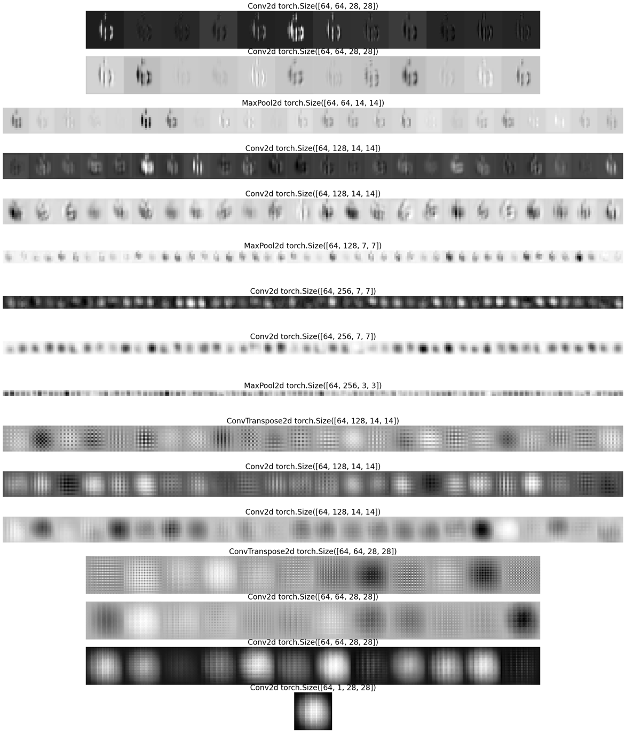
\includegraphics[width=\textwidth]{Figure/Front_page/mnist feature map.png}
    \caption{\textit{U-NET feature map for MNIST input}}
    \label{fig:mnist feature loss}
\end{figure}

\begin{figure}[H]
    \centering
    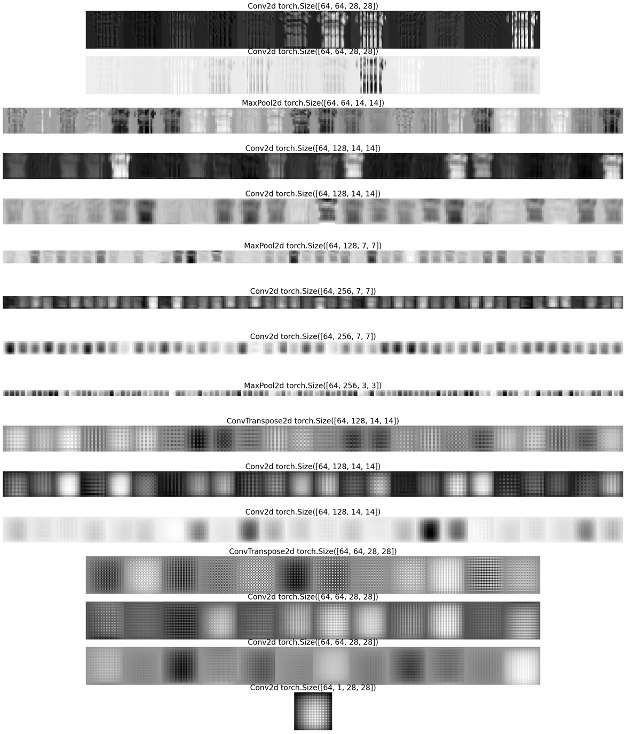
\includegraphics[width=\textwidth]{Figure/Front_page/fmnist feature map.png}
    \caption{\textit{U-NET feature map for F-MNIST input}}
    \label{fig:fmnist feature map}
\end{figure}